\section{REPL Commands}
\label{sec:commands}

To separate the implementation of user operations into logical units, each user
operation is encapsulated within a class implementing the
\texttt{IReplCommand} interface. See \cref{fig:uml-commands} for the design
of the \texttt{commands} package. After acquiring an invoker instance, the
frontend has two commands available by default:

\begin{description}
  \item [:load] \texttt{LanguageCommand}, loads a language from a file path;
  \item [:help] \texttt{HelpCommand}, prints descriptions of all available commands.
\end{description}

\begin{figure}[h]
  \centering
  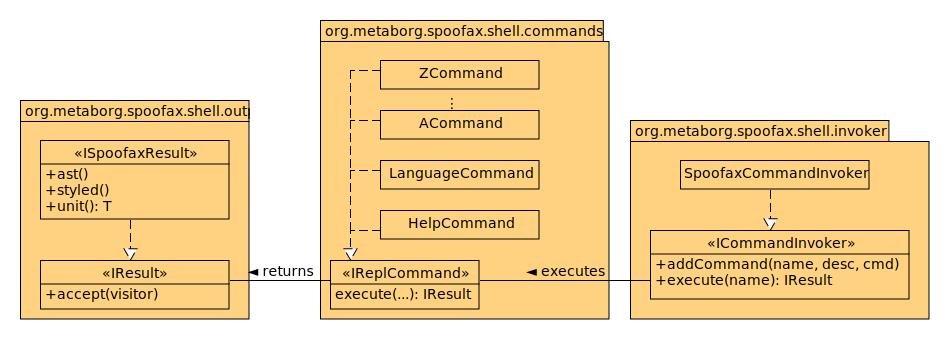
\includegraphics[width=\textwidth]{uml-commands}
  \caption{UML of the commands frontends can execute and the
           corresponding result interfaces.}
  \label{fig:uml-commands}
\end{figure}

Frontends can define additional commands by implementing the
\texttt{IReplCommand} interface.

As explained in the introduction of this chapter, there are only a few
commands that work across all languages, since every language can define its
own transformations or evaluation strategy. Therefore, the
\texttt{LanguageCommand} tries to determine several properties of the loaded
language and adjusts the set of loaded commands accordingly.

By splitting operations in small logical units the design ensures command
classes adhere to the Single Responsibility Principle, which makes all REPL
commands less complex and therefore easier to maintain. The logical units that
make up the commands also ensure a flexible design that can be modified
as the Spoofax architecture develops further on.

%%% Local Variables:
%%% TeX-master: "../main"
%%% End:
